\appendix
\renewcommand{\thesection}{\thechapter.\arabic{section}}
\chapter*{Anhang A}
\addcontentsline{toc}{chapter}{Anhang A \quad Mathematische Hintergründe und Herleitungen}
\markboth{Anhang A}{Anhang A}
\renewcommand{\thechapter}{A}
\renewcommand{\cftsecnumwidth}{3em}
\setcounter{chapter}{1}
\setcounter{section}{0}

\vspace{1em}
\begin{center}
	\LARGE\textbf{Mathematische Hintergründe und Herleitungen}
\end{center}




%\chapter*{Anhang A \quad Mathematische Hintergründe und Herleitungen}
%\addcontentsline{toc}{chapter}{Anhang A \quad Mathematische Hintergründe und Herleitungen}
%\renewcommand{\thechapter}{A}
%\setcounter{chapter}{1}


%\chapter{Mathematische Hintergründe und Herleitungen}
\label{chap:mathematische Hintergründe}
\markboth{}{}`        % entfernt Kapitelüberschrift in Kopfzeile
\thispagestyle{plain}
%\addcontentsline{toc}{chapter}{Mathematische Hintergründe und Herleitungen}

% Boxen-Stile definieren
\tcbset{physikbox/.style={colback=blue!5!white, colframe=blue!75!black, fonttitle=\bfseries}}
\tcbset{mathebox/.style={colback=green!5!white, colframe=green!50!black, fonttitle=\bfseries}}
\tcbset{didaktikbox/.style={colback=yellow!5!white, colframe=yellow!50!black, fonttitle=\bfseries}}
\tcbset{hypobox/.style={colback=orange!5!white, colframe=orange!75!black, fonttitle=\bfseries}}
\tcbset{hinweisbox/.style={colback=gray!10!white, colframe=black!40!black, fonttitle=\bfseries}}


\section{ Herleitung der Compton-Formel}
\subsubsection*{Ein Photon stößt auf ein Elektron}


\begin{center}
	\begin{tikzpicture}[scale=2, >=latex]
		
		% Achsen
		\draw[->] (-0.2,0) -- (3.5,0) node[right] {$x$};
		\draw[->] (0,-2.2) -- (0,2.2) node[above] {$y$};
		
		% Ursprung = Elektron vor Stoß
		\filldraw[blue] (0,0) circle (0.04) node[below left] {Elektron (ruhend)};
		
		% Einfallender Photon
		\draw[->, thick, blue] (-2,0) -- (0,0);
		\node[blue] at (-2.2, 0.2) {Photon einfallend $\vec{p}_\gamma$};
		
		% Elektron nach Stoß
		\draw[->, thick, blue] (0,0) -- (2,-1);
		\node[blue] at (0.8,-0.6) {$\vec{p'}_e$};
		\node[blue] at (2.2,-1.1) {Elektron nach Stoß};
		
		% Photon nach Stoß
		\draw[->, thick, red] (0,0) -- (1.3,2) ;
		\node[red] at (0.6,1.3){$\vec{p'}_\gamma$};
		\node[red] at (1.5,2.1) {Photon nach Stoß};
		
		% Winkel Theta (zwischen x-Achse und gestreutem Photon)
		%\draw (1,0) arc (0:-26.565:1);
		%\node at (1.2,-0.3) {$\theta$};
		
		% Optional: Winkel des Elektrons (phi)
		\draw (0.7,0) arc (0:57.995:0.7);
		\node at (0.75,0.3) {$\theta$};
		\node[blue] at (-0.2,0.2) {$\vec{p}_e$};
	\end{tikzpicture}
\end{center}



\subsubsection*{Energieübertragung beim Compton-Effekt}

Das einfallende Photon besitzt eine höhere Energie (und damit eine höhere Frequenz) als das gestreute Photon nach dem Stoß. Ein Teil der Photonenenergie wird auf das Elektron übertragen, wodurch das Photon Energie verliert. Da die Energie eines Photons proportional zur Frequenz ist,
\[
E = h \nu,
\]
verringert sich nach dem Stoß die Frequenz des gestreuten Photons – seine Wellenlänge wird entsprechend größer.

\subsubsection*{Die Energieerhaltung bei dem Stoß}
\[
E_\gamma + E_e = E'_\gamma + E'_e
\]

\begin{align*}
	E_\gamma :&\quad \text{Energie des einfallenden Photons} \\
	E_e       : &\quad \text{Energie des Elektrons vor dem Stoß } \\
	E'_\gamma  :&\quad \text{Energie des gestreuten Photons} \\
	E'_e       :&\quad \text{Energie des Elektrons nach dem Stoß }
\end{align*}
Zur Vereinfachung der Schreibweise wird definiert:\\
\begin{align*}
	p_\gamma &=	\mid   \overrightarrow{p}_\gamma\mid\\
	p_e &=	\mid   \overrightarrow{p}_e\mid\\
\end{align*}



\subsubsection*{Für das masseslose Photon gilt: }
\begin{align*}
	E_\gamma =\sqrt{m^2c^4+c^2p_\gamma^2}=cp_\gamma\quad \text{da m=0}
\end{align*}

\subsubsection*{Für das ruhende Elektron gilt: }
\begin{align*}
	E_e =m_ec^2
\end{align*}
\subsubsection*{Für das Photon nach dem Stoß  gilt: }
\begin{align*}
	E'_e =\sqrt{m_e^2c^4+c^2p_e^2}
\end{align*}
\subsubsection*{So ergibt sich für die Energieerhaltung}
\begin{align}
	E_\gamma + E_e&= E'_\gamma + E'_e\nonumber\\
	cp_\gamma+m_ec^2&=cp'_\gamma+\sqrt{m_e^2c^4+c^2{p'_e}^2} \label{Energie}
\end{align}
Gesucht: Beziehung zwischen $p_\gamma, p'_\gamma$ und den Winkel $\theta$. Also muss $p'_e$ eliminiert werden.\\
\subsubsection*{Für die Impulserhaltung gilt:}
Koordinatensystem geschickt gewählt:\\
\begin{itemize}
	\item Elektron im Ursprung
	\item Photon fliegt entlang der X-Achse direkt auf das Elektron
	
\end{itemize}
\begin{center}
	\begin{tikzpicture}[scale=2, >=latex]
		
		% Achsen
		\draw[->] (-0.2,0) -- (3.5,0) node[right] {$x$};
		\draw[->] (0,-2.2) -- (0,2.2) node[above] {$y$};
		
		% Ursprung = Elektron vor Stoß
		\filldraw[blue] (0,0) circle (0.04) node[below left] {Elektron (ruhend)};
		
		% Einfallender Photon
		\draw[->, thick, blue] (-2,0) -- (0,0);
		\node[blue] at (-2.2, 0.2) {Photon einfallend $\vec{p}_\gamma$};
		
		% Elektron nach Stoß
		\draw[->, thick, blue] (0,0) -- (2,-1);
		\node[blue] at (0.8,-0.6) {$\vec{p'}_e$};
		\node[blue] at (2.2,-1.1) {Elektron nach Stoß};
		
		% Photon nach Stoß
		\draw[->, thick, red] (0,0) -- (1.3,2) ;
		\node[red] at (0.6,1.3){$\vec{p'}_\gamma$};
		\node[red] at (1.5,2.1) {Photon nach Stoß};
		
		% Winkel Theta (zwischen x-Achse und gestreutem Photon)
		%\draw (1,0) arc (0:-26.565:1);
		%\node at (1.2,-0.3) {$\theta$};
		
		% Optional: Winkel des Elektrons (phi)
		\draw (0.7,0) arc (0:57.995:0.7);
		\node at (0.75,0.3) {$\theta$};
		\node[blue] at (-0.2,0.2) {$\vec{p}_e$};
	\end{tikzpicture}
\end{center}

\begin{align*}
	\overrightarrow{p_\gamma} +\overrightarrow{p_e}=&\overrightarrow{p'_\gamma}+\overrightarrow{p'_e}\\
\end{align*}
Daraus folgt dann:\\
\begin{align*}
	&\overrightarrow{p_\gamma}=\begin{pmatrix}p_\gamma\\0\\0 \end{pmatrix}\\
	&\overrightarrow{p_e}=\begin{pmatrix}0 \\0\\0 \end{pmatrix}\\
	&\overrightarrow{p'_\gamma}= \begin{pmatrix}p'_{\gamma x}  \\p'_{\gamma y}\\0 \end{pmatrix}\\
	&\overrightarrow{p'_e}=  \begin{pmatrix}p'_{ex} \\p'_{ey} \\0 \end{pmatrix}\\
\end{align*}
\begin{align*}
	\begin{pmatrix}p_\gamma\\0\\0 \end{pmatrix}+\begin{pmatrix}0 \\0\\0 \end{pmatrix}= \begin{pmatrix}p'_{\gamma x} \\p'_{\gamma y}\\0 \end{pmatrix}+  \begin{pmatrix}p'_{ex}\\p'_{ey} \\0 \end{pmatrix}\\
\end{align*}
Dies ergibt dann zwei Gleichungen:\\
\begin{align}
	p_\gamma=&p'_{\gamma x}+p'_{ex} \nonumber\\
	\Leftrightarrow \nonumber\\
	p'_{ex}&=p_\gamma-p'_{\gamma x} \label{pex}  \\
	0=&p'_{\gamma y}+p'_{e y} \nonumber\\
	\Leftrightarrow \nonumber\\
	p'_{ey}&=-p'_{\gamma y}\label{pe}
\end{align}
Ebenso gilt die Beziehung mit Phytagoras:\\
\begin{align}
	{p'}^2_e=	{p'}^2_{ex}+	{p'}^2_{ey}\label{p}
\end{align}
Jetzt \ref{pex} und \ref{pe} in \ref{p} einsetzen und die ergibt dann die Gleichung:\\
\begin{align}
	{p'}^2&=(p_\gamma-p'_{\gamma x})^2+(-p'_{\gamma y})^2 \nonumber\\
	&=p_\gamma^2-2p_\gamma p'_{\gamma x}+p'^2_{\gamma x}+p'^2_{\gamma y}\label{pp}
\end{align}
Jetzt den Winkel $\theta$ mittels den $\cos(\theta)$ ausdrücken und einfügen. Es gilt ja:\\

\begin{center}
	\begin{tikzpicture}[scale=2, >=latex]
		
		% Achsen
		\draw[->] (-0.2,0) -- (3.5,0) node[right] {$x$};
		\draw[->] (0,-0.2) -- (0,2.2) node[above] {$y$};
		
		
		
		
		
		
		
		% Photon nach Stoß
		\draw[->, thick, red] (0,0) -- (1.3,2) ;
		\node[red] at (0.6,1.3){$\vec{p'}_\gamma$};
		\node[red] at (1.5,2.1) {Photon nach Stoß};
		
		% Winkel Theta (zwischen x-Achse und gestreutem Photon)
		%\draw (1,0) arc (0:-26.565:1);
		%\node at (1.2,-0.3) {$\theta$};
		
		% Optional: Winkel des Elektrons (phi)
		\draw (0.7,0) arc (0:57.995:0.7);
		\node at (0.75,0.3) {$\theta$};
		
	\end{tikzpicture}
\end{center}
\begin{align}
	p'_{\gamma x} = p'_\gamma \cos (\theta) \label{winkel}
\end{align}
\ref{winkel} in \ref{pp} einsetzen und dies ergibt dann die zweite Gleichung die  in \ref{Energie} eingesetzt wird.\\
\begin{align}
	{p'}_e^2=p_\gamma^2-2p_\gamma p'_\gamma \cos (\theta)+p'^2_{\gamma y}\label{pp}
\end{align}
Hier nochmals die zwei Gleichungen \ref{Energie} und \ref{pp}:\\
\begin{align*}
	{p'}_e^2&=p_\gamma^2-2p_\gamma p'_\gamma \cos (\theta)+p'^2_{\gamma y}\\
	cp_\gamma+m_ec^2&=cp'_\gamma+\sqrt{m_e^2c^4+c^2{p'_e}^2} 
\end{align*}
Die Gleichung \ref{pp} wird in \ref{Energie} eingesetzt.\\
\begin{align*}
	cp_\gamma+m_ec^2&=cp'_\gamma+\sqrt{m_e^2c^4+c^2(p_\gamma^2-2p_\gamma p'_\gamma \cos (\theta)+{p'}^2_{\gamma y})} \\
	cp_\gamma+m_ec^2-cp'_\gamma&=\sqrt{m^2_ec^4+c^2p^2_\gamma+c^2{p'}^2_{\gamma y}-2c^2p_\gamma p'_\gamma \cos(\theta)}\quad \\
	(cp_\gamma+m_ec^2-cp'_\gamma)^2&=m^2_ec^4+c^2p^2_\gamma+c^2{p'}^2_{\gamma y}-2c^2p_\gamma p'_\gamma \cos(\theta)\\
	c^2p^2_\gamma+m_e^2c^4+c^2{p'}^2_\gamma+2m_ec^3p_\gamma-2c^2p_\gamma{p'}_\gamma-2m_ec^3p'_\gamma&=m^2_ec^4+c^2p^2_\gamma+c^2{p'}^2_{\gamma y}-2c^2p_\gamma p'_\gamma \cos(\theta)\\
\end{align*}


\begin{align*}
	\cancel{\color{red}c^2 p^2_\gamma}
	+ \cancel{\color{blue}m_e^2 c^4}
	+ \cancel{\color{teal}c^2 {p'}^2_\gamma}
	+ \color{orange}2 m_e c^3 p_\gamma
	- \color{purple}2 c^2 p_\gamma p'_\gamma
	- \color{cyan}2 m_e c^3 p'_\gamma
	&=
	\cancel{\color{blue}m_e^2 c^4}
	+ \cancel{\color{red}c^2 p^2_\gamma}
	+ \cancel{\color{teal}c^2 {p'}^2_{\gamma y}}
	- \color{purple}2 c^2 p_\gamma p'_\gamma \cos(\theta)
\end{align*}




Nach dem Kürzen bleibt:

\[
2 m_e c^3 p_\gamma - 2 m_e c^3 p'_\gamma = -2 c^2 p_\gamma p'_\gamma \cos(\theta) + 2 c^2 p_\gamma p'_\gamma
\]

Faktorisiere jeweils \( 2 m_e c^3 \) und \( 2 c^2 p_\gamma p'_\gamma \):

\[
2 m_e c^3 (p_\gamma - p'_\gamma) = 2 c^2 p_\gamma p'_\gamma (1 - \cos\theta)
\]

Nun nach \( p_\gamma - p'_\gamma \) auflösen:

\[
p_\gamma - p'_\gamma = \frac{c^2}{m_e c^3} \cdot p_\gamma p'_\gamma (1 - \cos\theta)
= \frac{1}{m_e c} \cdot p_\gamma p'_\gamma (1 - \cos\theta)
\]






\subsubsection*{Herleitung der Compton-Formel aus dem Impuls-Ausdruck}

Aus der Impuls-Gleichung nach dem Stoß gilt:
\[
p_\gamma - p'_\gamma = \frac{1}{m_e c} \cdot p_\gamma p'_\gamma (1 - \cos\theta)
\]

\subsubsection*{Zusammenhang zwischen Impuls und Wellenlänge}

Für Photonen (masselose Teilchen) gilt:
\[
E = h f = c p \quad \Rightarrow \quad p = \frac{h f}{c}
\]

Da \( c = \lambda f \), folgt:
\[
p = \frac{h}{\lambda}
\]


\subsubsection*{ Impulsdarstellung mit Wellenlänge}

Für Photonen setzen wir:
\[
p_\gamma = \frac{h}{\lambda}, \quad p'_\gamma = \frac{h}{\lambda'}
\]

Einsetzen in die Gleichung:

\[
\frac{h}{\lambda} - \frac{h}{\lambda'} = \frac{1}{m_e c} \cdot \frac{h}{\lambda} \cdot \frac{h}{\lambda'} (1 - \cos\theta)
\]

\subsubsection*{Gemeinsamer Nenner links}

\[
h \left( \frac{1}{\lambda} - \frac{1}{\lambda'} \right) = \frac{h^2}{m_e c \lambda \lambda'} (1 - \cos\theta)
\]

\subsubsection*{ Rechte Seite auf denselben Nenner bringen}

Multipliziere beide Seiten mit \( \lambda \lambda' \):

\[
h (\lambda' - \lambda) = \frac{h^2}{m_e c} (1 - \cos\theta)
\]

\subsubsection*{Durch \( h \) teilen}

\[
\lambda' - \lambda = \frac{h}{m_e c} (1 - \cos\theta)
\]

\subsubsection*{Endform: Die Compton-Formel}

\[
\boxed{
	\Delta \lambda = \lambda' - \lambda = \frac{h}{m_e c} (1 - \cos\theta)
}
\]




\subsection*{Folgerungen und Anwendungen der Compton-Formel}

Die Compton-Formel lautet:
\[
\Delta \lambda = \lambda' - \lambda = \frac{h}{m_e c}(1 - \cos\theta)
\]

Der maximale Wert ergibt sich für \( \theta = 180^\circ \), da hier \( 1 - \cos(180^\circ) = 2 \). Damit:

\[
\Delta \lambda_\text{max} = 2 \cdot \frac{h}{m_e c}
= 2 \cdot \frac{6{,}626 \cdot 10^{-34}~\text{Js}}{9{,}109 \cdot 10^{-31}~\text{kg} \cdot 3{,}0 \cdot 10^8~\text{m/s}}
= 4{,}85 \cdot 10^{-12}~\text{m}
\]

Diese Wellenlängenverschiebung ist nun im Vergleich zu verschiedenen Photonen-Wellenlängen zu betrachten:

\begin{center}
	\begin{tabular}{|l|c|c|c|}
		\hline
		\textbf{Strahlungsart} & \(\lambda\) [m] & \(\Delta \lambda\) [m] & \(\frac{\Delta \lambda}{\lambda}\) \\
		\hline
		Rotes Licht & \(7{,}0 \cdot 10^{-7}\) & \(4{,}85 \cdot 10^{-12}\) & \(6{,}93 \cdot 10^{-6}\) \\
		Röntgenstrahlung & \(1{,}0 \cdot 10^{-11}\) & \(4{,}85 \cdot 10^{-12}\) & \(0{,}485\) \\
		Gammastrahlung & \(1{,}0 \cdot 10^{-13}\) & \(4{,}85 \cdot 10^{-12}\) & \(48{,}5\) \\
		\hline
	\end{tabular}
\end{center}

\subsubsection*{Fazit}

Die Tabelle zeigt deutlich:

\begin{itemize}
	\item Bei sichtbarem Licht (z.\,B. rot, \( \lambda = 700\,\text{nm} \)) ist die relative Wellenlängenänderung durch den Compton-Effekt vernachlässigbar klein.
	\item Im Röntgenbereich ist \(\Delta \lambda\) vergleichbar mit der ursprünglichen Wellenlänge – der Effekt ist hier klar messbar.
	\item Für hochenergetische Gammastrahlung übersteigt \(\Delta \lambda\) sogar die ursprüngliche Wellenlänge um ein Vielfaches – der Compton-Effekt dominiert die Wechselwirkung mit Materie.
\end{itemize}

Dies erklärt auch, warum der Compton-Effekt ursprünglich bei der Untersuchung von Röntgenstrahlung entdeckt wurde – bei sichtbarem Licht wäre die Streuung durch Elektronen nicht nachweisbar.



\begin{figure}[h]
	\centering
	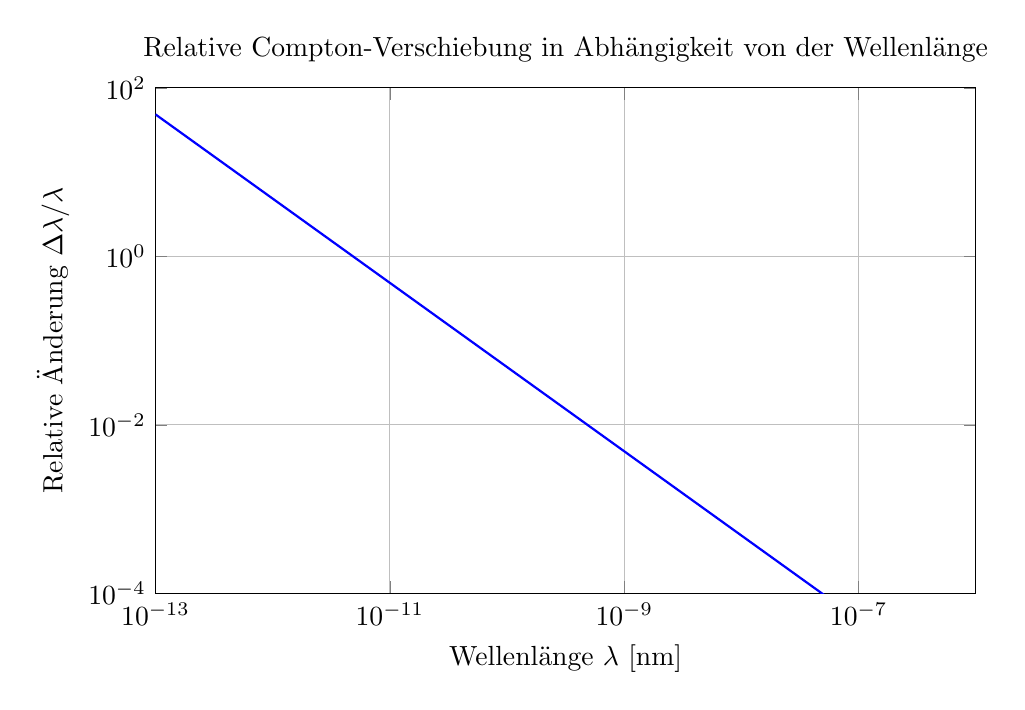
\begin{tikzpicture}
		\begin{axis}[
			width=12cm,
			height=8cm,
			xlabel={Wellenlänge $\lambda$ [nm]},
			ylabel={Relative Änderung $\Delta \lambda / \lambda$},
			title={Relative Compton-Verschiebung in Abhängigkeit von der Wellenlänge},
			xmode=log,
			ymode=log,
			grid=both,
			minor grid style={gray!20},
			major grid style={gray!50},
			domain=1e-13:1e-6,
			samples=500,
			xmin=1e-13, xmax=1e-6,
			ymin=1e-4, ymax=1e2,
			xtick={1e-13,1e-11,1e-9,1e-7},
			xticklabels={$10^{-13}$, $10^{-11}$, $10^{-9}$, $10^{-7}$},
			ytickten={-4,-2,0,2}
			]
			\addplot [
			thick,
			blue
			]
			expression {
				4.849416e-12 / x
			};
		\end{axis}
	\end{tikzpicture}
	\caption{Relative Wellenlängenänderung $\Delta \lambda / \lambda$ gemäß der Compton-Formel für $\theta = 180^\circ$ in Abhängigkeit von der einfallenden Wellenlänge $\lambda$.}
\end{figure}



\section{Lagrangedichte des elektromagnetischen Feldes}
% Struktur von F_{\mu\nu}, Bedeutung der Terme, Ableitung der Maxwell-Gleichungen

\section{Warum die Eichsymmetrie das Photon masselos macht}
% Transformation, Verbot des Masseterms, Argumentation mit Invarianz

\section{Transversalität des Photons aus Feldgleichungen}
% Freiheitsgrade des A^\mu, Lorentz-Eichung, Helizität

\section{Virtuelle Photonen in Feynman-Diagrammen}
% Unterschied real/virtuell, Beitrag zu Streuamplituden, keine physikalische Polarisationsprojektion

% Weitere optionale Abschnitte nach Be